\documentclass[10pt,letterpaper]{article}

% Self-contained source: figures, data, and references compile from this file.
\usepackage[margin=0.83in,top=0.88in,bottom=0.83in]{geometry}
\usepackage[T1]{fontenc}
\usepackage{lmodern}
\usepackage{microtype}
\usepackage{amsmath,amssymb}
\usepackage{booktabs,array,tabularx,multirow}
\usepackage{graphicx}
\usepackage{xcolor}
\usepackage{tikz}
\usetikzlibrary{arrows.meta,positioning,calc,fit}
\usepackage{pgfplots}
\pgfplotsset{compat=1.18}
\usepackage{hyperref}
\usepackage{fancyhdr}
\usepackage{titlesec}
\usepackage{enumitem}
\usepackage{caption}

\definecolor{ink}{HTML}{14243A}
\definecolor{muted}{HTML}{526276}
\definecolor{blue}{HTML}{155E86}
\definecolor{teal}{HTML}{158A84}
\definecolor{pale}{HTML}{EAF5F4}
\definecolor{rulegray}{HTML}{D8E2E8}
\definecolor{amber}{HTML}{BE7D22}
\hypersetup{colorlinks=true,linkcolor=blue,citecolor=blue,urlcolor=blue,pdftitle={Context Virtual Memory: Bounded Working Sets for Million-Object Agent Worlds},pdfauthor={CVM Project}}
\captionsetup{font=small,labelfont={bf,color=ink},textfont={color=muted}}
\titleformat{\section}{\Large\bfseries\color{ink}}{\thesection}{0.65em}{}
\titleformat{\subsection}{\large\bfseries\color{ink}}{\thesubsection}{0.55em}{}
\titlespacing*{\section}{0pt}{1.2em}{0.45em}
\titlespacing*{\subsection}{0pt}{0.9em}{0.3em}
\setlist[itemize]{leftmargin=1.25em,topsep=3pt,itemsep=1pt}
\setlength{\parindent}{0pt}
\setlength{\parskip}{5pt}
\setlength{\emergencystretch}{2em}
\pagestyle{fancy}
\setlength{\headheight}{19pt}
\fancyhf{}
\fancyhead[L]{\sffamily\footnotesize\color{muted} CVM / WORKING PAPER}
\fancyhead[R]{\sffamily\footnotesize\color{muted} OCTOBER 2026}
\fancyfoot[C]{\sffamily\footnotesize\color{muted} \thepage}
\renewcommand{\headrulewidth}{0.35pt}
\renewcommand{\headrule}{\hbox to\headwidth{\color{rulegray}\leaders\hrule height \headrulewidth\hfill}}

\newcommand{\stat}[2]{\begin{minipage}[t]{0.23\linewidth}\centering\sffamily\color{teal}\fontsize{18}{20}\selectfont\bfseries #1\\[-1pt]\color{muted}\fontsize{8}{10}\selectfont #2\end{minipage}}
\newcommand{\cvm}{\textsc{CVM}}
\newcommand{\op}[1]{\textsf{#1}}
\newcommand{\repo}[1]{\href{https://github.com/nikitph/2ter/blob/master/cvm/#1}{\texttt{#1}}}

\begin{document}
\thispagestyle{empty}
\vspace*{0.36in}
{\sffamily\bfseries\small\color{teal}\MakeUppercase{Systems study \quad / \quad Interim results}}\\[0.19in]
{\sffamily\bfseries\fontsize{29}{34}\selectfont\color{ink} Context Virtual Memory}\par
{\sffamily\fontsize{17}{23}\selectfont\color{blue} Bounded Working Sets for Million-Object Agent Worlds}\par
\vspace{0.14in}
{\color{rulegray}\rule{\linewidth}{0.7pt}}\par
{\sffamily\small\color{muted} CVM Project \hfill Working paper \;\textbullet\; 7 October 2026}\par
\vspace{0.14in}

\begin{abstract}
\noindent Agents need to investigate large external worlds without placing those worlds in the model prompt. We study \emph{Context Virtual Memory} (\cvm), a runtime that gives a model stable object handles, explicit page faults, bounded resident objects, durable notes, and evidence-checked answers. In a synthetic incident world growing from 112 to 999,991 objects, a deterministic prompt-only policy solves 90/90 tasks at each size while its mean peak resident set remains 8.1--9.4 objects and its estimated peak prompt remains 1.55--1.79k tokens. A live DeepSeek-V4.1-Flash processor solves 21/30 tasks at the largest size with 12.3 resident objects and a 1.97k-token estimated mean peak. A controlled reference-policy ablation shows that notes permit perfect accuracy with two resident objects; without notes, two-object accuracy is zero and re-fetching reaches 96\%. In a separate live-model test at one million objects, reducing residency from 32 to four objects lowers DeepSeek accuracy from 27/40 to 4/40, accompanied by 59\% re-fetching. We also report an interim Qwen2.5-7B-Instruct adapter: 252/256 exact actions on held-out trajectory states after 203 training steps, and a single successful end-to-end serving pilot. These results establish the behavior of this prototype and motivate larger paired model evaluations; they do not establish general world-size invariance or task-level improvement from fine-tuning.
\end{abstract}

\vspace{0.12in}
\colorbox{pale}{\parbox{\dimexpr\linewidth-2\fboxsep\relax}{\vspace{0.13in}
\stat{999,991}{largest world, objects}\hfill
\stat{1.79k}{reference peak prompt\textsuperscript{a}}\hfill
\stat{0.70}{live model accuracy, $n=30$}\hfill
\stat{4/40}{live accuracy at 4 objects}
\vspace{0.12in}}}\par
{\footnotesize\color{muted}\textsuperscript{a}Prompt sizes throughout are characters divided by four, not tokenizer counts.}

\section{The problem and the claim}

An agent can hold a tiny task in a huge world: ``find the change that caused this incident'' may require a handful of services and facts, even if the environment contains a million objects. Putting every object in a prompt makes cost scale with the world. Ordinary tools avoid that initial dump, but can return whole high-degree objects and leave an unbounded transcript. One-shot retrieval keeps prompts short while denying the agent the chance to choose the next lookup from newly discovered facts.

\cvm{} separates the world address space from the model's resident view. The runtime owns objects, access rights, replacement, and provenance. The model chooses where to look, which evidence to preserve, and when to answer. Our empirical question is whether \emph{useful behavior} survives a small resident view while the address space grows. A hard cap itself trivially bounds residency; the nontrivial observations are prompt size, accuracy, and re-fetching under that cap.

This paper reports two stages of evidence. V0 measures the substrate and a live model against growing synthetic worlds. V1 measures the four-object failure, constructs training and test data, and reports an unfinished model-training pilot. We present reference-policy and model results separately throughout.

\section{Mechanism}

Objects have stable URI-like handles. The model can \op{SEARCH} for discovery, \op{TRAVERSE} a named relation, and \op{FAULT} a known handle into the resident set. A least-recently-used policy evicts objects when the object or token budget is exceeded; the model cannot silently expand the set. \op{WRITE} stores short, evidence-linked notes in a separately bounded scratch area. \op{ANSWER} cites fact identifiers previously materialized in that context. The runtime checks namespace capabilities before operations and rejects answers with missing or unmaterialized citations. A rejected answer returns control for another step.

\begin{figure}[t]
\centering
\begin{tikzpicture}[font=\sffamily\small,>=Latex,node distance=7mm and 10mm]
\tikzset{box/.style={draw=rulegray,rounded corners=3pt,very thick,fill=white,align=center,minimum height=14mm}, flow/.style={-{Latex[length=2mm]},thick,color=blue}}
\node[box,minimum width=35mm] (model) {Model\\\footnotesize one operation / step};
\node[box,minimum width=51mm,right=16mm of model] (runtime) {CVM runtime\\\footnotesize capabilities $\cdot$ LRU $\cdot$ fact ledger};
\node[box,minimum width=34mm,right=16mm of runtime] (world) {External world\\\footnotesize objects + references};
\node[box,minimum width=46mm,below=13mm of runtime] (view) {Resident view + notes\\\footnotesize rebuilt prompt; no transcript};
\draw[flow] ([yshift=3mm]model.east) -- ([yshift=3mm]runtime.west);
\draw[flow] ([yshift=-3mm]runtime.west) -- ([yshift=-3mm]model.east);
\draw[flow] (runtime.east) -- (world.west);
\draw[flow] ([yshift=-3mm]world.west) -- ([yshift=-3mm]runtime.east);
\draw[flow] (runtime.south) -- (view.north);
\draw[flow] (view.west) -| ([xshift=-7mm]model.south) -- (model.south);
\end{tikzpicture}
\caption{The model issues operations to the runtime, which dereferences external objects and renders a bounded view for the next step. Handles remain usable after eviction; citations refer to fact-ledger entries, not to editable notes.}
\label{fig:system}
\end{figure}

Each model step receives a fresh rendering of task, resident objects, handles, notes, and rules. The previous conversation transcript is not carried forward. In this prototype, the default limit is 32 resident objects and a 16k-token estimated view budget; V1 also evaluates a four-object limit. A task may still use many \emph{total} tokens across many steps. The verifier establishes that cited identifiers were available, not that the model's inference from them is sound.

\section{Experimental design}

The primary synthetic world contains clusters of services, hosts, deployments, changes, metrics, incidents, people, teams, and claims. Shared platform services have increasing in-degree as the world grows. Tasks ask for an incident's root cause, the responsible owner, or whether a claim is supported or contradicted. They require multi-hop dereferences and include temporal and graph distractors. Task depth is one to three in V0. The generator increases \emph{world size} while keeping each sampled task's local causal chain roughly fixed. The result should therefore be read as a fixed-local-complexity study, not as a theorem for arbitrary graph queries.

The \emph{reference processor} is a deterministic policy that reads only the rendered prompt and emits one action. It has no direct access to the world store. It tests whether the interface carries enough information for a known-good policy; it is not an LLM. V0 compares it with full context, one-shot BM25, graph-expanded retrieval, and a tool-calling baseline that serializes whole objects and preserves the transcript. The latter is a specific by-value API design, not every possible tool design. V0 also runs DeepSeek-V4.1-Flash with a generic prompt, temperature zero, and at most 50 steps. All reported prompt sizes are characters divided by four; model API usage is reported separately in repository artifacts.

\section{V0: scaling the world}

\begin{figure}[t]
\centering
\begin{tikzpicture}
\begin{axis}[
 width=0.91\linewidth,height=58mm,
 xmode=log,ymode=log,log basis x=10,log basis y=10,
 xmin=90,xmax=1250000,ymin=900,ymax=200000,
 xtick={100,1000,10000,100000,1000000},
 xticklabels={$10^2$,$10^3$,$10^4$,$10^5$,$10^6$},
 ytick={1000,10000,100000},yticklabels={1k,10k,100k},
 grid=both,major grid style={draw=rulegray},minor grid style={draw=rulegray!45},
 xlabel={World objects},ylabel={Mean peak prompt, estimated tokens},
 legend style={draw=none,fill=none,font=\footnotesize,at={(0.01,0.98)},anchor=north west},
 tick label style={font=\footnotesize},label style={font=\small},
 ]
\addplot+[very thick,color=teal,mark=*,mark size=2.3pt] coordinates {(112,1547) (1015,1727) (10002,1732) (100001,1790) (999991,1793)};
\addlegendentry{CVM, reference policy}
\addplot+[very thick,color=amber,mark=square*,mark size=2.2pt] coordinates {(112,1491) (1015,1902) (10002,2798) (100001,12698) (999991,116229)};
\addlegendentry{Whole-object tool baseline}
\end{axis}
\end{tikzpicture}
\caption{In 90 reference-policy tasks per tier, CVM's peak prompt stays near 1.5--1.8k estimated tokens. The particular whole-object baseline grows when a lookup serializes the inverse edges of a shared hub. Logarithmic axes; token estimates are characters/4.}
\label{fig:scale}
\end{figure}

At five world sizes from 112 to 999,991 objects, the reference processor answers all 90 tasks per tier correctly. Mean peak residency stays between 8.1 and 9.4 objects; estimated peak prompts stay between 1,547 and 1,793 tokens (Figure~\ref{fig:scale}). At the largest size, the whole-object tool baseline also answers all tasks but reaches 116,229 estimated peak prompt tokens. A full-context rendering would require about 79 million estimated tokens at that size; it was not executed there. One-shot BM25 and graph-expanded retrieval score 0.21 and 0.30, respectively, at one million objects, but these are limited, untuned baselines and cannot establish superiority over stronger iterative retrieval.

The bounded view has a cost. At one million objects the reference policy takes about 30.5 steps and sends 34,835 estimated prompt tokens in total per task, compared with roughly 9.3 steps for whole-object tool calling. CVM wins on \emph{peak} context in this design; it does not minimize step count or total tokens at every scale. The tool baseline's growth is caused by serializing a high-degree hub. Returning paginated identifiers would remove much of that particular gap.

\begin{table}[t]
\centering\small
\caption{Live DeepSeek-V4.1-Flash with a 32-object limit. Means are per task. The two accuracy samples are small and use different tasks; the data do not establish equivalence across world sizes.}
\label{tab:live}
\begin{tabular}{lrr}
\toprule
 & 1,015 objects & 999,991 objects\\
\midrule
Tasks & 15 & 30\\
Correct & 8/15 (0.53) & 21/30 (0.70)\\
Mean peak resident objects & 11.5 & 12.3\\
Mean peak prompt, estimated tokens & 1,874 & 1,970\\
Mean steps & 28.2 & 29.9\\
Root-cause accuracy & 0.40 & 0.40\\
\bottomrule
\end{tabular}
\end{table}

The live-model loop retains bounded residency at both sizes (Table~\ref{tab:live}). Its larger-world accuracy is 21/30, compared with 8/15 in the smaller world. The samples are too small and unpaired to conclude that accuracy improves, or even to tightly bound any degradation. The unchanged 0.40 root-cause accuracy indicates that causal inference and distractor handling are substantial remaining errors. In these live runs, 18--26\% of attempted answers were rejected for unsupported citations and retried. No unsupported answer was accepted in the observed traces, but some accepted, cited answers were wrong.

\section{Memory pressure: what the notes do}

V0 switches \op{WRITE} notes on and off under the same deterministic policy at roughly one million world objects. With notes enabled, the processor scores 1.00 at resident limits of 2, 4, 8, and 32 objects with no re-fetches. With notes disabled, accuracy falls to 0.00 at two objects, 0.03 at four, and 0.33 at eight; re-fetch rates are 0.96, 0.90, and 0.58, respectively. At 16 or 32 objects, notes-disabled accuracy returns to 1.00. This is a controlled policy ablation: notes let the policy carry discoveries through eviction, but it does not measure what an untrained model would do if forced to write notes.

\begin{table}[t]
\centering\small
\caption{V1 live-model test at 999,991 objects: 40 paired seeded tasks, generic prompt, 50-step limit. The four-object reference check uses 30 tasks and a different processor, so its 1.00 is a solvability control rather than a paired model estimate.}
\label{tab:tight}
\begin{tabular}{lrrr}
\toprule
 & DeepSeek, 32 objects & DeepSeek, 4 objects & Reference, 4 objects\\
\midrule
Accuracy & 27/40 (0.68) & 4/40 (0.10) & 30/30 (1.00)\\
Mean peak resident objects & 12.7 & 3.9 & 4.0\\
Re-fetch rate & 0.00 & 0.59 & 0.00\\
Notes per task & 1.0 & 0.95 & 11.6\\
Step-limit hits & 3/40 & 22/40 & 0/30\\
\bottomrule
\end{tabular}
\end{table}

V1 then tests the pressure on the \emph{same live model and seeded tasks}. DeepSeek drops from 27/40 correct with 32 objects to 4/40 with four; 59\% of materializations re-fetch an evicted object, and 22/40 tasks hit the step limit (Table~\ref{tab:tight}). The model writes about one note per task in either condition; the reference processor writes about 12 and succeeds at four objects. Underuse of notes is a plausible explanation for thrashing, supported by the reference ablation. It is not a causal estimate for DeepSeek: the policies also differ in navigation and answer selection. A direct intervention on the same live model remains necessary.

\section{V1: training an operation policy}

The V1 exporter runs 10,000 solved reference tasks through the runtime and produces 254,147 training and 50,897 validation prompt/action examples. The world seeds are disjoint across these splits. Examples cover world sizes near $10^2$--$10^4$, three task kinds, depth 1--3, multiple resident limits, and 6,427 recovery targets after invalid answers, denied actions, useless faults, or evictions. This data teaches individual actions from reference trajectories; successful imitation does not by itself imply successful autonomous rollouts.

Seven held-out split generators pass 100/100 reference tasks each, including one-million-object scaling, depth 4--5, traps, a four-object tight split, and a code-repository domain. The second domain uses its own reference policy only as a solvability check; it contributes no training examples and has not yet been evaluated with a live model.

We fine-tune Qwen2.5-7B-Instruct with a rank-32 LoRA adapter. The saved artifact is checkpoint 203 of a planned 1,563 optimizer steps, about 13\% of the scheduled epoch. On the same 256 held-out reference-state prompts used for earlier gates, checkpoint 203 emits valid JSON on 255/256, chooses the right operation on 253/256, and matches the exact action on 252/256. In a separate operation-stratified 128-prompt check, it matches 67/69 \op{SEARCH} actions and 56/59 \op{ANSWER} actions exactly. These samples assess local imitation of a known trajectory distribution. They do not test error recovery after the model's own mistakes.

A paired serving smoke test uses one held-out four-object task at 999,991 world objects. The base model reaches the 60-step limit without solving it and writes no notes. The step-203 adapter solves it in 30 steps, writes 12 notes, and stays at or below four residents. This is \emph{one task}, a check that serving and evaluation work, not an accuracy estimate or evidence of general improvement. Full base-versus-adapter task-level cells are pending.

\section{Relationship to prior work}

MemGPT introduced virtual context management for language-model agents and a hierarchy between limited immediate context and larger external memory~\cite{memgpt}. MEM1 studies compact model-maintained state across long multi-turn tasks~\cite{mem1}. ClawVM describes harness-managed memory pages, residency, provenance, and thrash metrics for agent sessions~\cite{clawvm}. CVM's mechanisms draw from this line of systems work. Its emphasis here is empirical: an explicit address space of external world objects; measured resident view against \emph{world size}; and a notes ablation under tight object caps. These differences are a description of this prototype's study, not a claim that paging or agent memory is new.

\section{Limits and decisive next tests}

The world is synthetic and designed with task-local causal chains. The reference processor is task-specific, so perfect reference accuracy is a capacity check, not evidence of general model ability. The live size comparison has only 15 and 30 tasks and uses different draws. All ``prompt token'' numbers in the scaling plots are approximate characters/4, and the whole-object and one-shot retrieval baselines leave design and tuning space. The verifier checks citation availability, not semantic entailment; grounded answers can be wrong. The adapter's 98.4\% exact-action result is conditional on reference states, while its end-to-end comparison has $n=1$. A code-repository domain is reference-tested only.

The most informative next experiment is a preregistered, paired base-versus-adapter rollout across world sizes and resident limits, with at least 100 tasks per cell, confidence intervals, and failure analysis. A direct model-side note intervention would test the proposed cause of four-object thrashing. A stronger by-reference tool baseline and iterative retrieval baseline would show whether CVM's runtime contracts confer benefits beyond API shape. Finally, a real graph or service topology and a faithfulness audit of retried citations would test generality and answer validity.

\section{Conclusion}

The prototype demonstrates that a model can navigate a million-object address space through a small resident view, and that a deterministic policy can preserve accuracy under a severe object cap when it records useful notes. In the current live model, the four-object setting exposes a sharp failure: repeated materialization and too little retained state. Early imitation training reproduces reference actions and passes a single serving smoke test. The systems result is a measured separation between world size and resident prompt size in these tasks; the open question is how reliably a learned policy can exploit that separation across models and domains.

\section*{Artifacts and reproducibility}

Code, experiment commands, raw summaries, and traces are in the \href{https://github.com/nikitph/2ter}{2ter repository}: \texttt{cvm/RESULTS\_V0.md}, \texttt{cvm/RESULTS\_V1.md}, \texttt{cvm/results/}, and \texttt{cvm/experiments/}. V1's full generated training set is about 1.9\,GB and is ignored by Git; \texttt{experiments/export\_trajectories.py} regenerates it from the recorded seed policy. The Runpod training checkpoint is retained on a network volume; the paper reports only results already recorded in the repository. The local test suite had 41 passing tests at this snapshot.

\begin{thebibliography}{9}
\bibitem{memgpt} C. Packer et al. \emph{MemGPT: Towards LLMs as Operating Systems}. arXiv:2310.08560, 2023. \url{https://arxiv.org/abs/2310.08560}.
\bibitem{mem1} A. Zhou et al. \emph{MEM1: Learning to Synergize Memory and Reasoning for Efficient Long-Horizon Agents}. arXiv:2506.15841, 2025. \url{https://arxiv.org/abs/2506.15841}.
\bibitem{clawvm} M. Rafique and L. Bindschaedler. \emph{ClawVM: Harness-Managed Virtual Memory for Stateful Tool-Using LLM Agents}. arXiv:2604.10352, 2026. \url{https://arxiv.org/abs/2604.10352}.
\end{thebibliography}

\end{document}
